\scanpage{28}

% The list and its long rules share a single coordinate field.
% Coordinates follow the supplied whole image, in original pixels.
% No written title, date, or manuscript sheet number is visible.
\figure{%
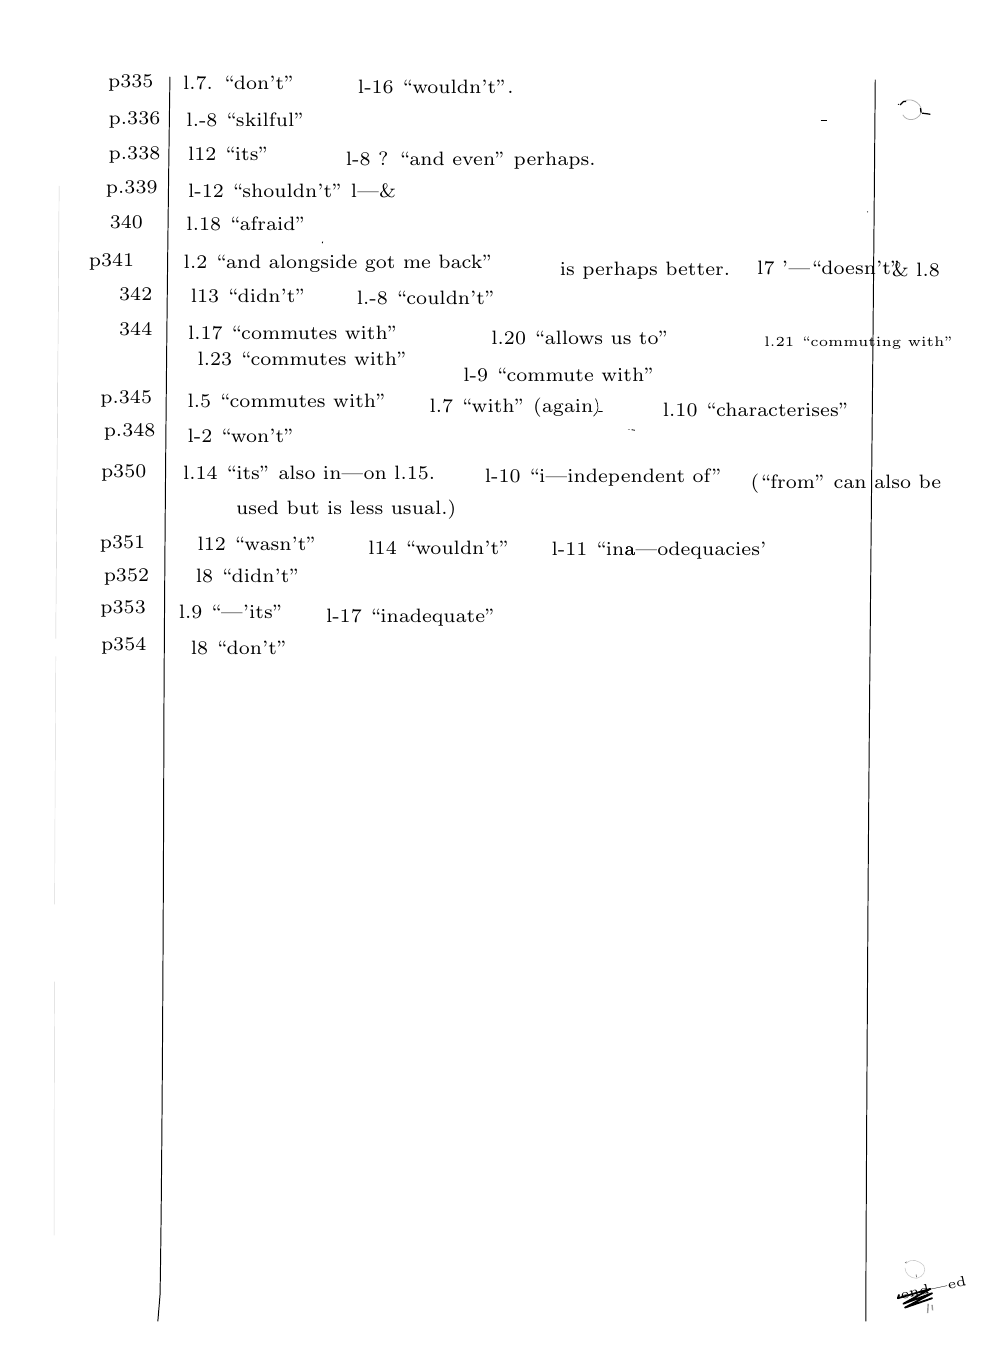
\begin{tikzpicture}[x=.007cm,y=-.007cm,every node/.style={anchor=base west,inner sep=0pt,font=\scriptsize}]
\path[use as bounding box] (0,0) rectangle (1688,2362);
% 335
\node at (145,109) {p335};
\node at (281,113) {l.7. ``don't''};
\node at (598,120) {l-16 ``wouldn't''.};
% 336
\node at (146,176) {p.336};
\node at (287,180) {l.-8 ``skilful''};
% 338: the question and the qualification are both live.
\node at (146,239) {p.338};
\node at (290,241) {l12 ``its''};
\node at (576,250) {l-8 ? ``and even'' perhaps.};
% 339
\node at (141,300) {p.339};
\node at (290,308) {l-12 ``shouldn't'' \deleted{\unsure{l|\&}}};
% 340
\node at (148,364) {340};
\node at (287,367) {l.18 ``afraid''};
% 341. The reference to l.8 and the closing quote of doesn't extend right of the rule.
\node at (110,433) {p341};
\node at (282,436) {l.2 ``and alongside \uline{got me} back''};
\node at (964,449) {is perhaps better.};
\node at (1322,447) {l7 \unsure{'|``}doesn't''};
\node at (1566,451) {\& l.8};
% 342
\node at (165,495) {342};
\node at (295,499) {l13 ``didn't''};
\node at (596,502) {l.-8 ``couldn't''};
% 344: two physical lines form one page-reference block.
\node at (165,558) {344};
\node at (290,565) {l.17 ``commutes with''};
\node at (840,574) {l.20 ``allows us to''};
\node[font=\tiny] at (1335,578) {l.21 ``commuting with''};
\node at (307,612) {l.23 ``commutes with''};
\node at (789,641) {l-9 ``commute with''};
% 345. The short stroke attached to the right parenthesis is drawn as seen;
% whether it functions as a full stop is not settled.
\node at (131,681) {p.345};
\node at (289,689) {l.5 ``commutes with''};
\node at (728,697) {l.7 ``with'' (again\tikz[baseline=0pt,x=1ex,y=1ex]{\draw[line width=.08ex,line cap=round] (.10,1.6) .. controls (.53,.8) and (.52,.05) .. (-.12,-.48);\draw[line width=.08ex,line cap=round] (.46,.04)--(.92,.04);}};
\node at (1151,706) {l.10 ``characterises''};
% 348
\node at (137,741) {p.348};
\node at (289,752) {l-2 ``won't''};
% 350. Dense returned strokes below the initial i remain doubted as in C.
\node at (132,816) {p350};
\node at (281,820) {l.14 ``its'' also \unsure{in|on} l.15.};
\node at (828,825) {l-10 ``\unsure{\uuline{i}|\uline{i}}ndependent of''};
\node at (1310,835) {(``from'' can also be};
\node at (377,882) {used but is less usual.)};
% 351. The old and live bodies occupy one physical letter position.
\node at (130,944) {p351};
\node at (307,949) {l12 ``wasn't''};
\node at (617,955) {l14 ``wouldn't''};
\node at (949,957) {l-11 ``in\tikz[baseline=(oldA28C.base)]{\node[inner sep=0pt] (oldA28C) {\deleted{\unsure{a|o}}};\node[anchor=base west,inner sep=0pt] at (oldA28C.base west) {a};}dequacies'};
% 352
\node at (137,1005) {p352};
\node at (304,1007) {l8 ``didn't''};
% 353
\node at (131,1063) {p353};
\node at (273,1072) {l.9 \unsure{``|'}its''};
\node at (540,1078) {l-17 ``inadequate''};
% 354
\node at (132,1129) {p354};
\node at (295,1136) {l8 ``don't''};
% Main left and right rules; they continue through the otherwise blank lower field.
\draw[line width=.35pt] (258,89) .. controls (253,447) and (249,858) .. (247,1261) .. controls (246,1686) and (243,2145) .. (240,2298) -- (236,2346);
\draw[line width=.35pt] (1537,94) .. controls (1533,596) and (1527,1127) .. (1524,1562) .. controls (1522,1889) and (1520,2210) .. (1520,2346);
% Faint discontinuous trace at the far left, without an assigned textual role.
\draw[black!20,line width=.16pt] (57,287) .. controls (56,493) and (53,795) .. (51,1108);
\draw[black!15,line width=.16pt] (51,1140) .. controls (50,1358) and (49,1493) .. (49,1590);
\draw[black!16,line width=.16pt] (49,1730) .. controls (48,1904) and (48,2040) .. (48,2190);
% Upper-right ring-like trace and its dark parts; physical origin is unassigned.
\draw[black!30,line width=.3pt] (1590,133) .. controls (1605,125) and (1625,141) .. (1620,155) .. controls (1613,169) and (1594,171) .. (1587,158);
\draw[line width=.45pt] (1582,140)--(1588,134)--(1593,134) (1619,146)--(1620,154) (1622,155)--(1637,157);
\fill (1579,139) circle[radius=1.1];
\draw[line width=.35pt] (1438,169)--(1449,169);
% Small isolated marks in the written field; no punctuation role is supplied.
\fill (1523,334) circle[radius=1.1];
\draw[line width=.3pt] (535,388)--(534,391);
\draw[black!40,line width=.3pt] (1088,728)--(1093,728);
\draw[line width=.3pt] (1095,729)--(1101,730);
% Faint lower-right ring-like trace above the cancelled note.
\draw[black!20,line width=.22pt] (1593,2241) .. controls (1602,2231) and (1616,2235) .. (1625,2245) .. controls (1630,2255) and (1624,2265) .. (1612,2268) .. controls (1600,2268) and (1591,2259) .. (1591,2249);
\draw[black!55,line width=.25pt] (1591,2240)--(1594,2238) (1611,2261)--(1612,2266);
% Bottom-right margin note, slanting upwards to the right and wholly cancelled.
\node[rotate=12,font=\tiny,anchor=base west] (end28C) at (1584,2306) {\deleted{\unsure{end|ed}}};
\draw[line width=.65pt,line cap=round,line join=round] (1580,2298)--(1578,2304)--(1637,2287)--(1588,2314)--(1640,2295)--(1591,2321)--(1640,2304);
\draw[black!40,line width=.5pt] (1633,2314)--(1632,2331) (1640,2316)--(1641,2326);
\end{tikzpicture}%
}

% archive sheet number: 27
